\documentclass[a4paper, 1.5lines]{ctexart}
\usepackage[top=3cm, bottom=2cm]{geometry}
\usepackage{graphicx}
\usepackage{subcaption}
\usepackage{amsmath}
\usepackage{xcolor}
\usepackage{url}
\usepackage{booktabs}
\usepackage{multirow}
%\usepackage{hyperref}
\usepackage[hidelinks]{hyperref} % 加载 hyperref 并隐藏链接边框

%\usepackage[utf8]{inputenc}
%\usepackage[ngerman]{babel} % 加载德语支持

% booktabs 提供 \toprule, \midrule, \bottomrule 等表格命令
\usepackage{booktabs}
% 定义占位命令以避免未定义控制序列错误
\newcommand{\placeholderspace}{}
\usepackage{fancyhdr} % 导入fancyhdr宏包
\usepackage{lipsum}   % 仅用于生成示例文本
\usepackage{float}    % 提供 H 浮动位置选项

% 设置页面样式为fancy
\pagestyle{fancy}
% 自定义页眉内容
\fancyhead[L]{} % 左侧页眉
\fancyhead[C]{\textbf{Physics-experiment Reporting Letter:\\Zeeman Effect}} % 中间页眉
\fancyhead[R]{ } % 右侧页眉
% 自定义页脚内容
\fancyfoot[L]{ } % 左侧页脚
\fancyfoot[C]{\thepage} % 中间页脚显示页码
\fancyfoot[R]{ } % 右侧页脚
% 改变页眉线的粗细
\renewcommand{\headrulewidth}{1.4pt}
% 改变页脚线的粗细
\renewcommand{\footrulewidth}{0.pt}





\title{塞曼效应}
\author{实验人：学生\qquad 学号：[学号已脱敏]\qquad 指导教师：蒋楠}
\date{实验日期：2025.12.4}


\begin{document}
    
    \maketitle
    
    \begin{abstract}
         本实验采用法布里–珀罗标准具结合 CCD 成像系统，对汞灯谱线在外加磁场作用下产生的塞曼分裂现象进行了观测与分析。实验首先利用毫特斯拉计探头对电磁铁所产生磁场进行标定，获得了磁感应强度与励磁电流之间的$ B\!-\!I$ 关系曲线。在此基础上，分别记录了汞绿线与汞黄线在无磁场及施加磁场条件下的干涉环分布，并对各谱线干涉环的直径及其偏振性质进行了测量。实验结果表明，对于同一波长的谱线，其相邻级次干涉圆环的直径平方差保持恒定；在发生塞曼分裂后，$\sigma$线与 $\pi $线表现出彼此正交的偏振方向。进一步通过测定谱线分裂间距反推出对应的磁场强度，发现由光谱分裂计算得到的磁场值整体上大于毫特斯拉计的直接测量结果。
        
         \textbf{\textbf{关键词：塞曼效应\quad 汞绿线\quad 汞黄线\quad 法布里-珀罗标准具}}
    \end{abstract}
    
    \section{引言}
        塞曼效应是物理学发展史中的一个重要里程碑，其发现和解释过程清晰地反映了物理理论由经典框架向量子理论体系的演进。1896 年，荷兰物理学家塞曼首次在实验中观测到原子谱线在磁场中的分裂现象，即所谓的正常塞曼效应；随后，洛伦兹基于经典电磁理论对这一现象给出了合理解释。然而，对于后来发现的反常塞曼效应，经典理论已无法充分说明，直到电子自旋这一量子自由度被引入，人们才对其物理机制形成完整认识。塞曼效应的研究不仅加深了对原子内部结构和量子力学基本规律的理解，也在天体物理、原子物理以及材料科学等多个研究领域中获得了重要应用。

        在本实验中，将借助法布里–珀罗标准具对汞绿线（546.1 nm）和汞黄线（579.0 nm）在外加磁场中的谱线分裂进行观测，重点分析分裂后谱线的间距变化及其偏振特性，从而验证塞曼效应的基本规律。
    \section{原理}
        将原子光源置于外加磁场中时，原本发射的单色谱线会发生分裂，并呈现出具有特定偏振方向的多条谱线结构。谱线分裂的条数及其分布形式与参与跃迁的能级类型密切相关，这一现象即为塞曼效应。

\subsection{物理原理——磁场引入的相互作用项}

当外磁场 $\vec{B}$ 存在时，电子（电荷量 $e$、质量 $m_e$）的能量将受到磁相互作用的影响，其哈密顿量在无磁场情形的基础上增加一项与角动量耦合的磁相互作用能。若取磁场方向沿 $\hat{z}$ 轴，则该附加项可写为
\begin{align}
\hat{H}_z & = \frac{e}{2m_e} \vec{B} \cdot (\vec{L} + 2\vec{S}),
\end{align}
其中 $\vec{L}$ 与 $\vec{S}$ 分别表示电子的轨道角动量和自旋角动量。该相互作用项使得原先关于磁量子数 $m_j$ 的简并能级发生劈裂，对应的能量修正为
\begin{equation}
E_z(j) = \frac{\hbar e B}{2 m_e} g m_j ,
\end{equation}
式中 $g$ 为朗德因子，其近似表达式为
\begin{equation}
g \approx 1 + \frac{j(j+1)+s(s+1)-l(l+1)}{2j(j+1)} .
\end{equation}

对于从初态 $a$ 跃迁至终态 $b$ 的辐射过程，若两态对应的朗德因子分别为 $g_a$、$g_b$，磁量子数为 $m_a$、$m_b$，则跃迁能量将产生$\Delta E = \frac{\hbar e B}{2 m_e} (g_a m_a - g_b m_b)$
的变化。将其换算为波数形式，可得谱线的波数偏移
\begin{equation}
\Delta \tilde{\nu} = \tilde{L} ( g_a m_a - g_b m_b ),
\end{equation}
其中
\centerline{$\tilde{L} = \frac{eB}{4\pi m c} \approx 0.467 B$}
称为洛伦兹单位，$\tilde{L}$ 的单位为 $\mathrm{cm}^{-1}$，磁场 $B$ 的单位为 T。

电偶极跃迁的选择定则要求 $\Delta m_j = 0, \pm 1$。由于跃迁前后原子角动量发生变化，辐射光必须携带相应的角动量，从而表现出明确的偏振性质。在垂直于磁场方向进行观测时，发射光均为线偏振光，其中
\begin{itemize}
\item $\Delta m = 0$：电矢量方向平行于磁场，称为 $\pi$ 线；
\item $\Delta m = +1$：电矢量方向垂直于磁场，称为 $\sigma^+$ 线；
\item $\Delta m = -1$：电矢量方向垂直于磁场，称为 $\sigma^-$ 线。
\end{itemize}

\subsubsection{汞绿线与汞黄线的塞曼分裂特征}

本实验选取汞绿线（546.1 nm）和汞黄线（579.0 nm）作为研究对象，其对应的能级跃迁关系如图 \ref{fig:tran} 所示。汞绿线的跃迁过程中同时涉及轨道角动量与自旋角动量，属于反常塞曼效应，在磁场中分裂为 9 条谱线，相邻谱线之间的波数差为 $\tilde{L}/2$。而汞黄线的跃迁仅与轨道角动量相关，对应正常塞曼效应，其谱线分裂为 3 条，相邻分量的波数间隔为 $\tilde{L}$。

\subsection{法布里–珀罗标准具的分光原理}

法布里–珀罗标准具由两块相互平行、具有高反射率的平面玻璃板构成，中间由间隔圈保持固定间距 $d$。当光以角度 $\theta$ 入射时，不同光程的多次反射光发生多光束干涉，满足相长干涉条件
\begin{equation}
2 d \cos \theta = K \lambda ,
\end{equation}
其中 $K$ 为干涉级次。该装置利用干涉角度对波长的依赖性实现高分辨率分光，但其观测效果也受到仪器分辨率和自由光谱范围的限制。

\textit{分辨本领}\qquad 多光束干涉条纹的锐利程度可用精细度 $F$ 表征，其定义为
\begin{equation}
F = \frac{\pi \sqrt{R}}{1 - R},
\end{equation}
其中 $R$ 为反射率。精细度越大，干涉条纹越窄、越清晰，仪器能够分辨的谱线数目也越多。

\textit{自由光谱范围}\qquad 由于不同波长的光可能对应不同干涉级次，若级次发生重叠将导致谱线难以区分。定义在干涉条纹中心附近不发生重叠时允许的最大波长差为自由光谱范围：
\begin{equation}
\Delta \lambda = \frac{\lambda^2}{2d},
\end{equation}
对应的波数形式为
\begin{equation}
\Delta \tilde{\nu} = \frac{1}{2d}.
\end{equation}

\begin{figure}[h!]
        \centering
        \begin{subfigure}{0.47\textwidth}
            \centering
            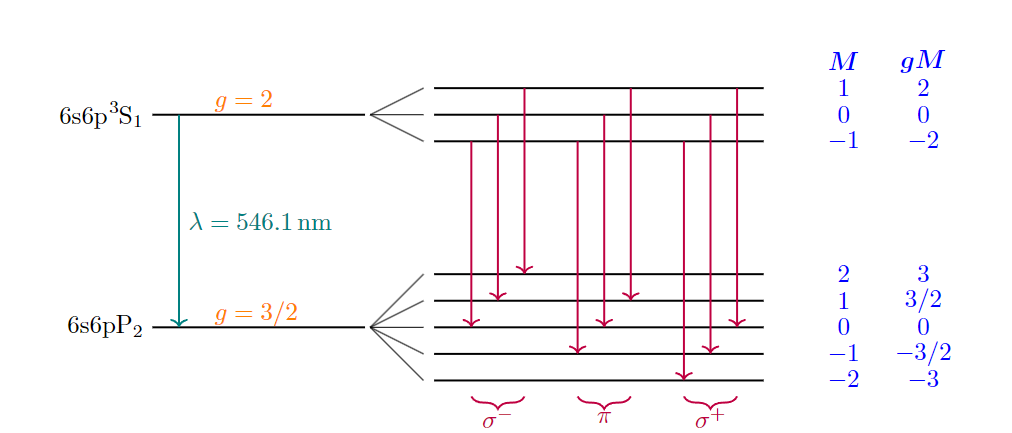
\includegraphics[width=\textwidth]{fig//transition1}
            \caption{546.1 nm汞绿线的能级跃迁}
            \label{key}
        \end{subfigure}
        \hfill
        \begin{subfigure}{0.47\textwidth}
            \centering
            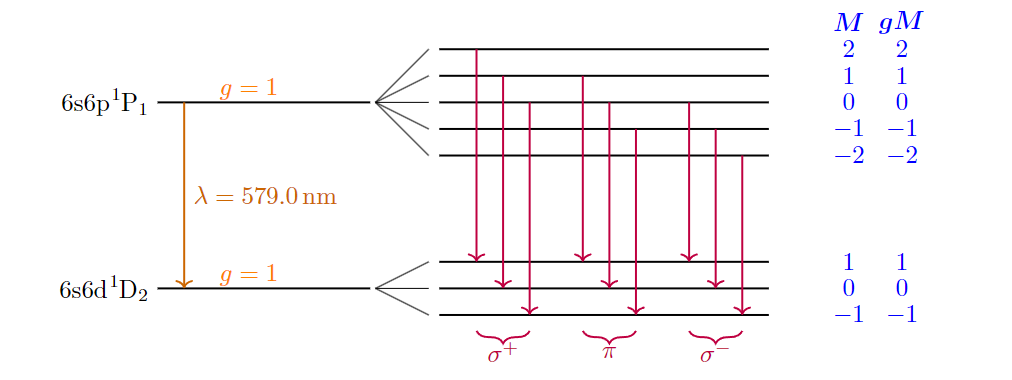
\includegraphics[width=\textwidth]{fig//transition2}
            \caption{579.0nm汞黄线的能级跃迁}
            \label{key}
        \end{subfigure}
        \caption{汞绿线和汞黄线对应的能级跃迁图}
        \label{fig:tran}
    \end{figure}
    \section{实验}
    \subsection{实验仪器}

\textbf{电磁铁与毫特斯拉计}\qquad
实验中通过电磁铁产生可调匀强磁场，并采用毫特斯拉计对磁场强度进行测量。改变通入电磁铁线圈的电流大小即可调节磁场强度。毫特斯拉计探头内部集成霍尔元件，磁场作用下产生与磁感应强度成正比的霍尔电压，从而实现对磁场的定量测量。

\textbf{汞灯光源}\qquad
汞灯作为实验光源，应精确放置在电磁铁轴线的中心位置，以保证其处于磁场最均匀的区域。在电磁铁外侧加装遮光罩以限制杂散光输出，同时需要合理调整汞灯与会聚透镜之间的距离，使进入后续光学系统的光束近似为平行光。

\textbf{滤光片}\qquad
实验中配备绿色和黄色两种滤光片，分别用于选取汞绿线和汞黄线，从而避免其他谱线对塞曼分裂观测的干扰。

\textbf{偏振片}\qquad
偏振片放置于法布里–珀罗标准具之前。通过连续旋转偏振片，可选择性地消去特定偏振方向的光，从而分别观察 $\sigma$ 线和 $\pi$ 线的消光现象，用于判定分裂谱线的偏振性质。

\textbf{会聚透镜}\qquad
会聚透镜位于 F-P 标准具之前，用于对入射光进行扩束处理，使干涉条纹在成像平面上分布得更加充分，有利于提高测量精度。

\textbf{光阑}\qquad
光阑用于检验光路的准直情况，同时可调节入射光强，以获得对比度较高、条纹较为锐利的干涉图样。

\textbf{CCD 摄像元件}\qquad
CCD 器件用于记录干涉条纹图像，其工作原理是将入射光的空间强度分布转换为电荷分布，从而实现对光学信号空间结构的快速、整体采集。

\textbf{光路示意图}

\begin{figure}[h!]
\centering
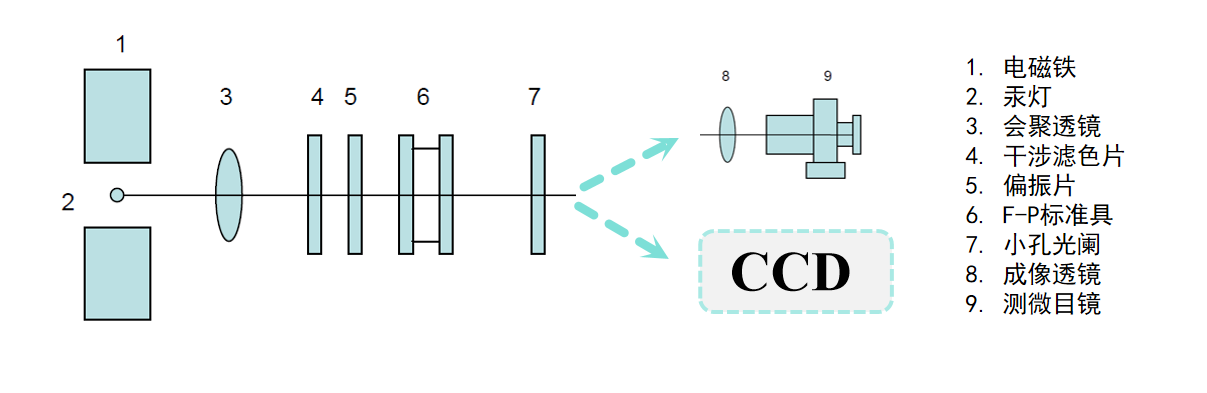
\includegraphics[width=15cm,height=5cm]{fig//equip}
\caption{实验光路示意图}
\label{key}
\end{figure}

\subsection{实验操作及主要内容}

\subsubsection{磁场的标定}

实验中磁场由电磁铁产生，磁感应强度通过毫特斯拉计探头进行测量。磁场大小由通入电磁铁的电流决定，控制主机设有“电压”和“电流”两种工作模式，并分别配有粗调和细调旋钮。其中电压档位用于限制最大电流值，显示屏直接给出电流读数，单位为毫安（mA）。

毫特斯拉计探头的核心元件为霍尔片，其测量原理基于经典霍尔效应。需要注意的是，霍尔效应只能测量与载流子运动方向垂直的磁场分量，且霍尔元件对磁场方向具有固定取向，因此在实际测量时必须严格调整探头的放置方向。此外，为了使磁场标定结果能够与后续由塞曼分裂谱线反演得到的磁场进行比较，探头位置应与汞灯位置保持一致，通常均放置在电磁铁轴线的中心区域。

在正式标定之前，需对毫特斯拉计进行调零操作。随后控制电流按 $0,\mathrm{A} \rightarrow 5,\mathrm{A} \rightarrow 0,\mathrm{A}$ 的顺序变化，在电流上升与下降过程中分别记录磁场强度，从而获得完整的 $B$–$I$ 标定曲线。

\subsubsection{光路的调整}

在实验开始前需对整个光路进行精细调节，以保证光束准直、干涉条纹对称且清晰。通过依次调整汞灯位置、会聚透镜、光阑以及 F-P 标准具的相对位置，使 CCD 成像平面上能够观察到均匀分布的同心圆干涉条纹，为后续测量奠定基础。

\subsubsection{汞绿线塞曼分裂谱的测量}

在光路调节完成后，首先在无外加磁场条件下记录干涉条纹，测量同一波长下相邻干涉级次条纹的直径平方差，以验证其为常数关系。

随后逐渐增大通入电磁铁的电流，使汞绿线在磁场中发生塞曼分裂。随着磁场强度的变化，谱线的分裂情况也随之改变：当电流较小时，分裂间距过小，谱线无法分辨；当电流过大时，不同干涉级次的条纹会发生重叠，从而影响判读。因此，只有在这两种情况之间的适当电流范围内，才能清晰观测并测量塞曼分裂谱线。

在不同电流条件下，记录对应的干涉条纹分布，并测量各条纹的直径，通过计算条纹直径平方差得到谱线的分裂间距。同时，在 F-P 标准具前放置偏振片并缓慢旋转，当某些谱线出现消光现象时记录偏振片的角度读数，以判断对应谱线的偏振方向。

通过上述方法，在不同外加磁场条件下求得谱线的塞曼分裂间隔，并进一步反推出相应的磁场强度，将其与磁场标定所得结果进行比较分析。

\textbf{汞黄线塞曼分裂谱的测量过程与汞绿线的测量步骤完全相同。}

        
    \section{结果与分析讨论}
        \subsection{磁场的标定}

在进行正式谱线测量之前，首先对电磁铁中心附近的磁场分布进行了初步探测。实验发现，电磁铁轴线中心处的磁场强度相较于周围区域呈现出局部极小值的特征。

此外，在未通电流的条件下对毫特斯拉计进行了调零操作。完成磁场测量并将探头移出电磁铁后，发现仪器仍给出一个非零但很小的磁感应强度读数。这表明实验所用电磁铁在长期使用后产生了不可忽略的\textbf{剩磁}，该因素在后续数据分析中需要加以考虑。

磁场标定结果如图 \ref{fig:biaoding} 所示。在电流 $0\sim3\,\mathrm{A}$ 范围内，磁场强度与电流之间呈现良好的线性关系；当电流超过 $3\,\mathrm{A}$ 后，磁场随电流的变化开始明显偏离线性。其可能原因在于：随着电流增大，线圈的焦耳热效应、磁滞效应等非理想因素逐渐增强，使部分磁场能量被耗散，磁感应强度的增长趋势趋于饱和。

\begin{figure}[h!]
    \begin{subfigure}{0.87\textwidth}
        \centering
        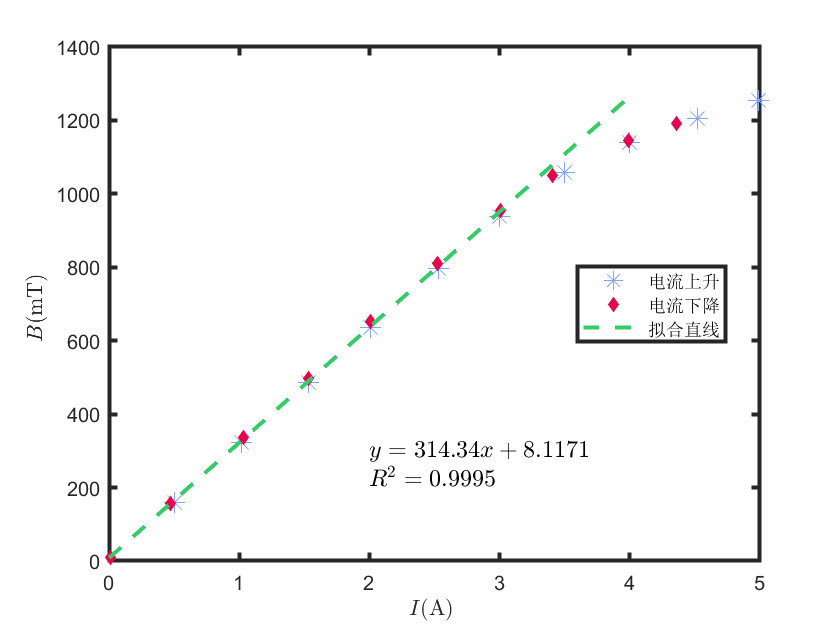
\includegraphics[width=\textwidth]{fig//BI_biaoding}
        \caption{磁场 $B$--$I$ 曲线的标定结果。电流按 $0\,\mathrm{A} \rightarrow 5\,\mathrm{A} \rightarrow 0\,\mathrm{A}$ 的顺序变化，在上升与下降过程中分别采集数据。图中“*”与菱形符号分别表示上升段与下降段数据点，直线为 $0\sim3\,\mathrm{A}$ 区间内的数据拟合结果。}
        \label{fig:biaoding}
    \end{subfigure}
    \hfill
    \begin{subfigure}{0.87\textwidth}
        \centering
        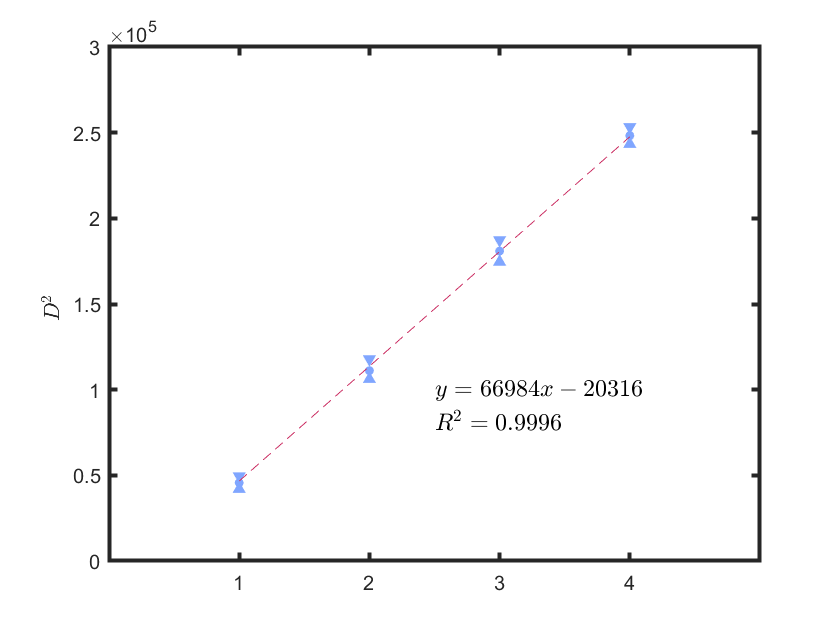
\includegraphics[width=\textwidth]{fig//D_square}
        \caption{干涉条纹直径平方与级次之间线性关系的验证。圆点对应以条纹中心为基准的数据，三角形对应以内、外边缘为基准的数据。为便于展示，令 $K,K-1,K-2,K-3$ 分别对应横坐标 $1,2,3,4$，线性拟合结果良好。}
        \label{fig:pingfang}
    \end{subfigure}
    \caption{实验数据的拟合结果}
    \label{key}
\end{figure}

\subsection{零磁场下的测量}

在无外加磁场条件下，对汞绿线的干涉条纹进行了测量。实验结果表明，同一波长下相邻干涉级次圆环直径的平方差为近似常数，其测量数据如下：

\begin{table}[h!]
    \centering
    \caption{零磁场下汞绿线的干涉条纹数据（直径单位：像素）}
    \label{tab:data}
    \begin{tabular}{|c|c|c|c|c|}
    \hline
    级次 & $K$ & $K-1$ & $K-2$ & $K-3$ \\
    \hline
    $D$ & 213.733 & 333.300 & 425.310 & 498.307 \\
    \hline
    $D^2$ & 45681.7 & 111089 & 180889 & 248310 \\
    \hline
    \end{tabular}
    \hfill
    \begin{tabular}{|c|c|c|c|}
    \hline
    相邻级次 & $K-1\rightarrow K$ & $K-2\rightarrow K-1$ & $K-3\rightarrow K-2$ \\
    \hline
    $\Delta D^2$ & 65407.2 & 69799.7 & 67420.9 \\
    \hline
    \end{tabular}
\end{table}

考虑到软件自动识别圆环与条纹边界的拟合效果有限，上表中的 $\Delta D^2$ 数值均经过适当修正，具体修正方法见附录说明。

另一方面，相邻级次直径平方差保持恒定意味着 $D^2$ 随级次呈线性变化关系。图 \ref{fig:pingfang} 中的拟合结果清晰地验证了直径平方与干涉级次之间的线性依赖。

\subsection{汞绿线塞曼分裂光谱的测量}

\subsubsection{谱线分裂现象}

如前所述，汞绿线在磁场中发生反常塞曼效应，原本单一的谱线将分裂为九条子谱线。实验表明，仅在一定磁场范围内才能对分裂谱线进行有效观测。不同电流条件下的实验结果如图 \ref{fig:range_of_I} 所示：当电流为 $1.54\,\mathrm{A}$ 时，谱线开始出现清晰分裂；当电流增大至 $4.63\,\mathrm{A}$ 时，不同干涉级次的条纹已发生明显重叠。

\begin{figure}[h!]
    \centering
    \begin{subfigure}{0.3\textwidth}
        \centering
        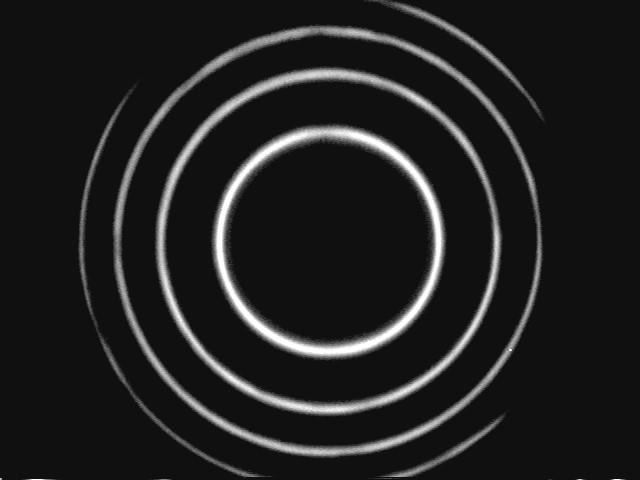
\includegraphics[width=\textwidth]{fig//zero//Hg0}
        \caption{$I=0\,\mathrm{A}$}
    \end{subfigure}
    \hfill
    \begin{subfigure}{0.3\textwidth}
        \centering
        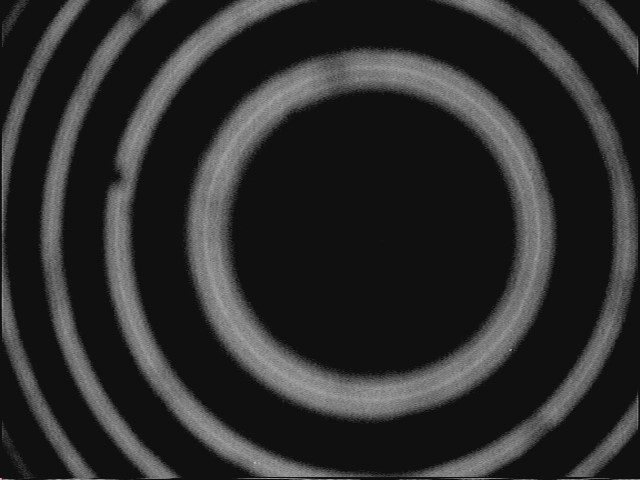
\includegraphics[width=\textwidth]{fig//green//Hg1_I_1.54A}
        \caption{$I=1.54\,\mathrm{A}$}
    \end{subfigure}
    \hfill
    \begin{subfigure}{0.3\textwidth}
        \centering
        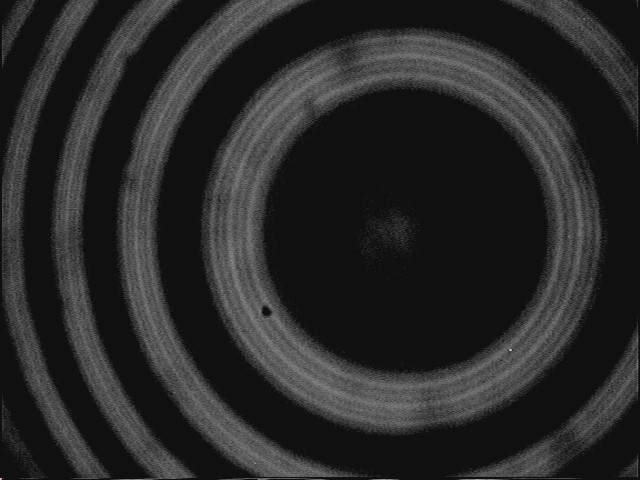
\includegraphics[width=\textwidth]{fig//green//Hg1_I_2.35A}
        \caption{$I=2.35\,\mathrm{A}$}
    \end{subfigure}
    \hfill
    \begin{subfigure}{0.3\textwidth}
        \centering
        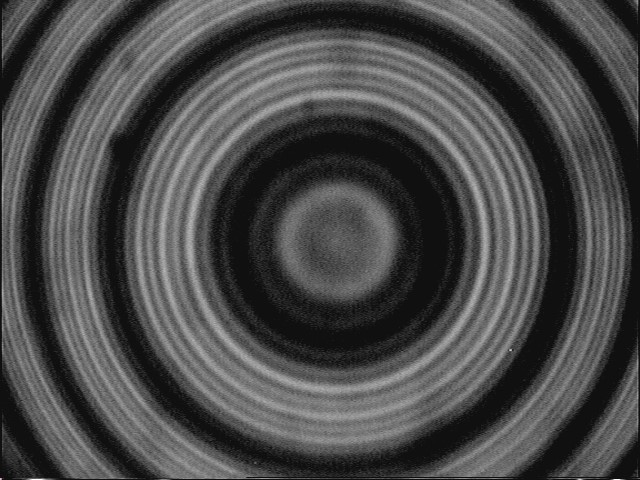
\includegraphics[width=\textwidth]{fig//green//Hg1_I_3.28A}
        \caption{$I=3.02\,\mathrm{A}$}
    \end{subfigure}
    \hfill
    \begin{subfigure}{0.3\textwidth}
        \centering
        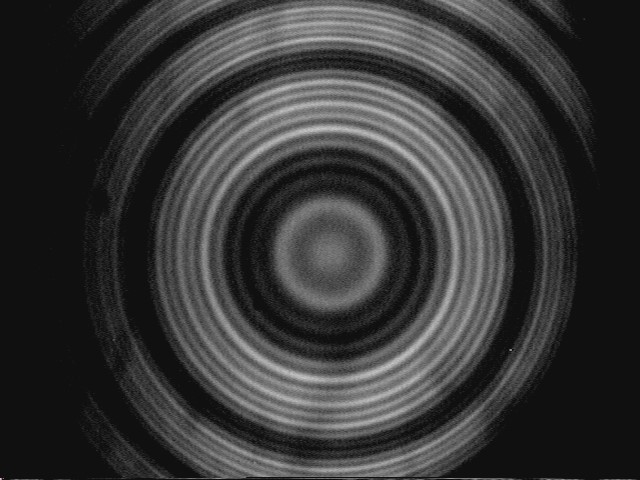
\includegraphics[width=\textwidth]{fig//green//Hg1_I_3.62A}
        \caption{$I=3.62\,\mathrm{A}$}
    \end{subfigure}
    \hfill
    \begin{subfigure}{0.3\textwidth}
        \centering
        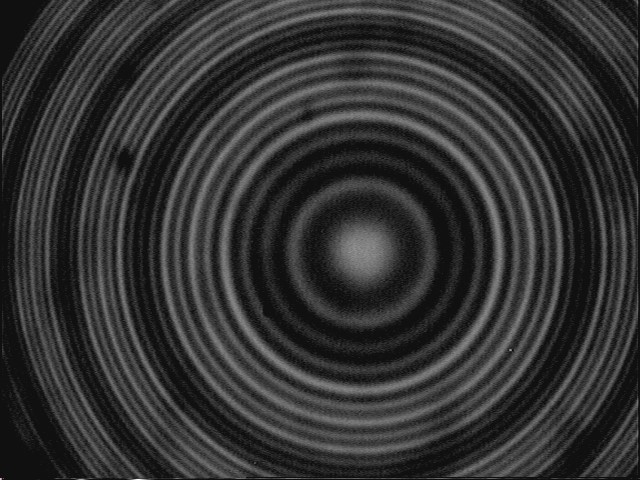
\includegraphics[width=\textwidth]{fig//green//Hg1_I_4.63A}
        \caption{$I=4.63\,\mathrm{A}$}
    \end{subfigure}
    \caption{不同磁场条件下汞绿线的塞曼分裂光谱}
    \label{fig:range_of_I}
\end{figure}

\subsubsection{谱线的偏振特性}

在电流为 $3.62\,\mathrm{A}$ 时，通过旋转偏振片观察谱线的消光现象，结果如图 \ref{fig:xiaoguang} 所示。当偏振片角度为 $\theta_1=217^\circ$ 时，$\sigma$ 光发生消光，仅剩三条 $\pi$ 线，其中中心 $\pi$ 线的位置与零磁场条件下的谱线一致；当偏振片角度转至 $\theta_2=131^\circ$ 时，$\pi$ 光消光，此时每个干涉级次内仅能观测到四条 $\sigma$ 线，其余两条由于强度过弱未能被清晰记录。

消光现象表明各子谱线均为线偏振光，而两种消光角度相差约 $90^\circ$，说明 $\sigma$ 光与 $\pi$ 光的偏振方向相互正交。

\subsubsection{由光谱反演磁场强度}

将汞绿线的实验数据代入式 (\ref{formula:calcu})，可由谱线分裂间距反推出对应的磁场强度，其结果与毫特斯拉计的直接测量值进行比较，如图 \ref{fig:comp} 所示。

\begin{figure}[h!]
    \centering
    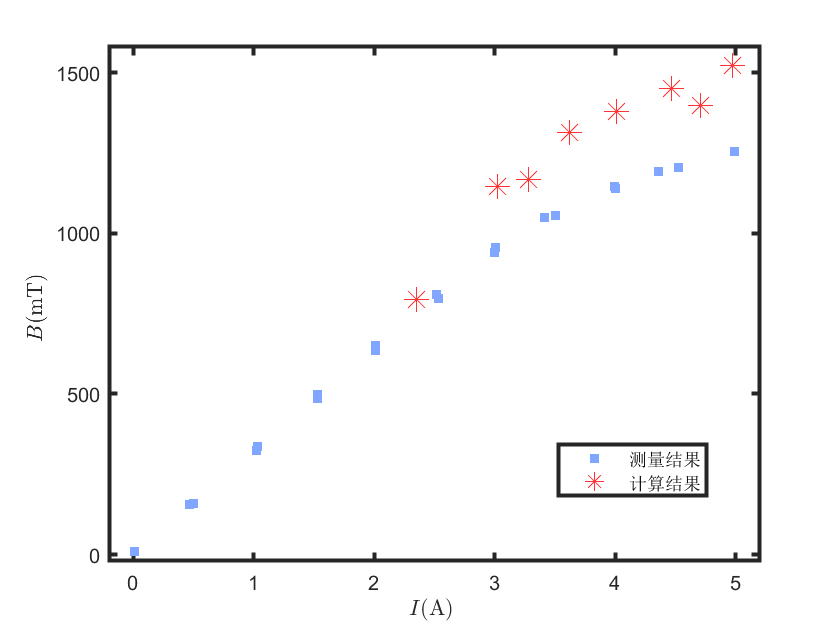
\includegraphics[width=0.92\textwidth]{fig//BI_comparasion}
    \caption{磁场测量值与由塞曼分裂计算得到的磁场结果对比}
    \label{fig:comp}
\end{figure}

其中正方形数据点表示毫特斯拉计的测量结果，星号表示由塞曼分裂计算得到的磁场值。可以看到，计算结果整体偏大，其主要原因可能在于霍尔探头的取向难以保证与磁场方向完全一致。由于霍尔效应只能测量磁场的特定分量，实际测得的磁场值往往小于真实磁场强度。

\subsubsection{误差来源与条纹特征讨论}

{\large \textit{两种磁场测量方法的误差来源}}

\begin{enumerate}
    \item 毫特斯拉计测量误差
    \begin{itemize}
        \item 电磁铁中心附近磁场分布并非完全均匀，探头位置偏差会引入系统误差；
        \item 电源输出电流存在波动，导致磁场产生随机误差；
        \item 霍尔元件的温度漂移影响其输出特性。
    \end{itemize}
    \item 塞曼分裂计算误差
    \begin{itemize}
        \item 圆环直径的测量依赖人工定标与程序处理，存在随机误差；
        \item CCD 成像平面与焦平面不完全重合，使干涉条纹偏离理想圆形；
        \item 谱线本身不够细锐，引入测量不确定度；
        \item 理论推导中所采用的近似忽略了部分高阶效应。
    \end{itemize}
\end{enumerate}

{\large \textit{干涉条纹的实际特征}}

实验中观察到部分光谱圆环存在局部缺失，同时同一圆环的亮度分布并不均匀。前者可能源于光学元件表面的污染或遮挡，后者则主要与背景光未完全消除有关。

\subsection{汞黄线塞曼分裂谱线的测量}

汞黄线发生正常塞曼效应，单条谱线在磁场中分裂为三条。实验确定其可测电流范围为 $0.68\,\mathrm{A}\sim2.88\,\mathrm{A}$。在 $I=0.86\,\mathrm{A}$ 条件下对谱线的偏振性质进行了验证：当偏振片角度为 $\theta_1=227^\circ$ 时，$\sigma$ 光消光；当偏振片角度为 $\theta_2=312^\circ$ 时，$\pi$ 光消光。

\begin{figure}[h!]
    \centering
    \begin{subfigure}{0.32\textwidth}
        \centering
        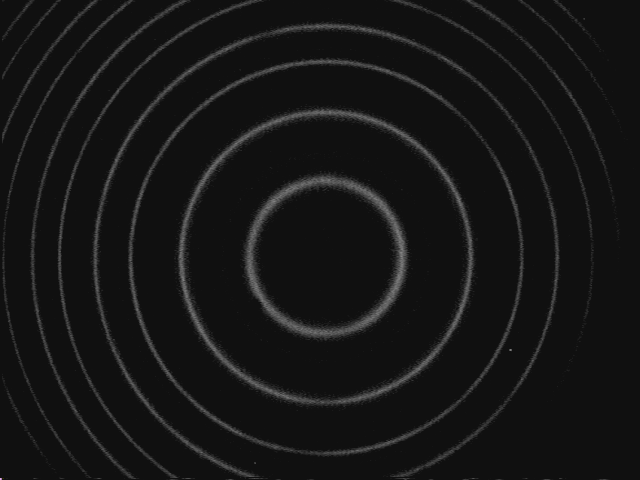
\includegraphics[width=\textwidth]{fig//zero//Hg2}
        \caption{$I=0\,\mathrm{A}$}
    \end{subfigure}
    \hfill
    \begin{subfigure}{0.32\textwidth}
        \centering
        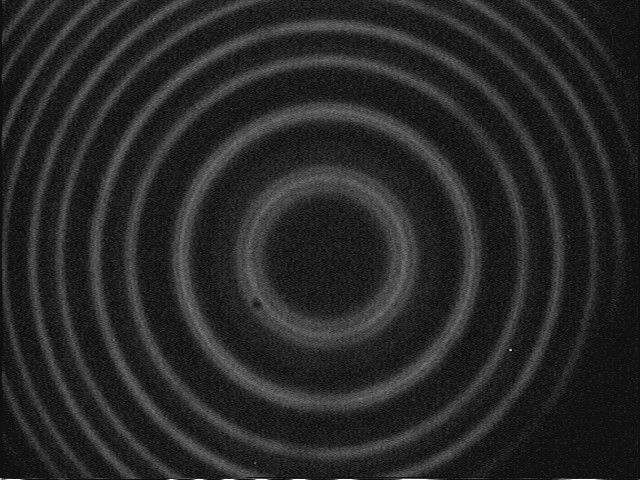
\includegraphics[width=\textwidth]{fig//yellow//Hg2_lowbound}
        \caption{$I=0.86\,\mathrm{A}$}
    \end{subfigure}
    \hfill
    \begin{subfigure}{0.32\textwidth}
        \centering
        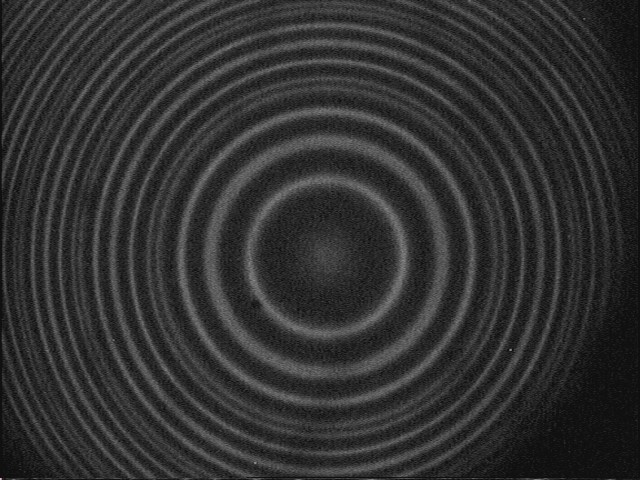
\includegraphics[width=\textwidth]{fig//yellow//Hg2_highbound}
        \caption{$I=2.88\,\mathrm{A}$}
    \end{subfigure}
    \caption{不同磁场下汞黄线的塞曼分裂光谱}
    \label{fig:ran_of_I}
\end{figure}

\begin{figure}[h!]
    \centering
    \begin{subfigure}{0.47\textwidth}
        \centering
        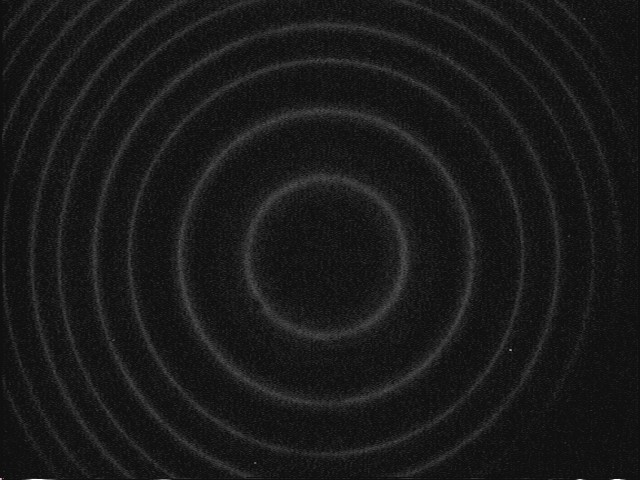
\includegraphics[width=\textwidth]{fig//yellow//Hg2_0.86A_227degree}
        \caption{$\sigma$ 光消光（$\theta=227^\circ$）}
    \end{subfigure}
    \hfill
    \begin{subfigure}{0.47\textwidth}
        \centering
        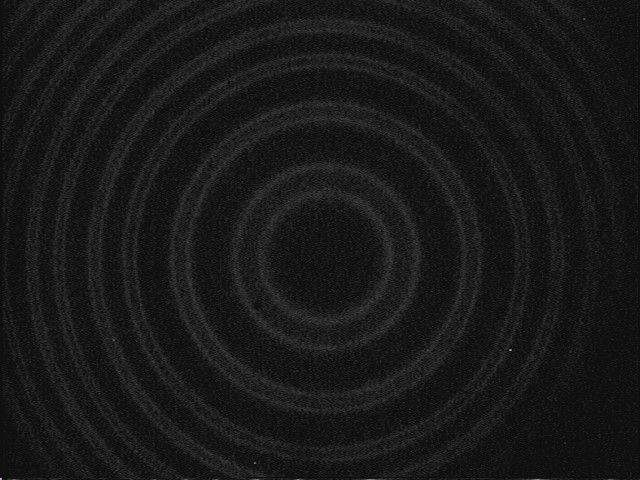
\includegraphics[width=\textwidth]{fig//yellow//Hg2_0.86A_312degree}
        \caption{$\pi$ 光消光（$\theta=312^\circ$）}
    \end{subfigure}
    \caption{汞黄线谱线的偏振特性验证}
    \label{fig:xiaohuang}
\end{figure}

实验中未能清晰分辨汞黄双线结构，推测其原因在于双线间距过小，已超出本实验装置的分辨能力，仅表现为谱线的整体展宽。
    \section{总结}
        在本实验中，我们借助法布里--珀罗标准具与 CCD 成像系统，对汞灯谱线在外加磁场中的塞曼分裂现象进行了系统观测。首先标定了电磁铁的磁场--电流关系，结果表明在 \(0\sim 3\) A 的电流范围内，磁场与电流呈现良好的线性依赖；而当电流进一步增大时，由于磁路逐渐进入饱和区，磁场强度开始偏离线性增长。随后，通过零磁场条件下汞绿线干涉条纹的测量，验证了同一波长谱线相邻级次圆环直径平方差 \(\Delta D^2\) 为常数这一理论预期。

在施加磁场后，我们观察到汞绿线发生反常塞曼分裂，谱线分裂为 9 条，而汞黄线则表现为正常塞曼效应，对应分裂为 3 条。结合偏振片的转动实验，确认了分裂后的谱线为两组偏振方向彼此正交的线偏振光。进一步利用 \(\Delta D^2\) 进行定标，计算了相邻分裂谱线的波数差，并由此反推出对应的磁场强度。将该结果与毫特斯拉计的标定值进行比较后发现，光谱计算得到的磁场值整体上大于直接测量结果，这一差异可以由磁场测量中探头取向及方向性误差等因素加以解释。

需要指出的是，实验中 CCD 所记录的谱线清晰度有限，谱线并不十分细锐，且位于外侧的干涉环常常部分超出视场范围，这在一定程度上影响了圆环直径的准确测量，从而显著放大了磁场反演结果的不确定性。从图 \ref{fig:comp} 可以看出，计算得到的磁场数据存在较为明显的波动，甚至出现了随电流增大而磁场反而减小的异常点。今后可通过改进成像质量和优化条纹直径的提取方法来降低这一误差。

此外，本实验未能清晰分辨汞黄双线，这可能与双线间距过小及系统分辨率不足有关。后续实验中可考虑提高光源强度或采用分辨率更高的光学与成像系统，以期获得更加完整和精细的谱线结构。
    \begin{thebibliography}{99}
        \bibitem{1}
        北京师范大学物理实验教学中心. 近代物理实验讲义一 (2019)
    \end{thebibliography}

    
\end{document}